\documentclass[aspectratio=169,11pt]{beamer}
\usepackage[T1]{fontenc}
\usepackage{lmodern,amsmath,amssymb,mathtools,bm,booktabs,array,graphicx,tikz}
\usetikzlibrary{arrows.meta,positioning,calc,decorations.pathreplacing,patterns}
\definecolor{ink}{HTML}{17344D}\definecolor{accent}{HTML}{087E8B}\definecolor{pale}{HTML}{EDF5F5}\definecolor{gold}{HTML}{AD6B19}
\providecommand{\dd}{\,\mathrm{d}}\providecommand{\R}{\mathbb{R}}
\providecommand{\E}{\mathbb{E}}\providecommand{\Var}{\operatorname{Var}}
\providecommand{\Cov}{\operatorname{Cov}}\providecommand{\diag}{\operatorname{diag}}
\providecommand{\norm}[1]{\left\lVert#1\right\rVert}
\providecommand{\abs}[1]{\left|#1\right|}
\usefonttheme{professionalfonts}
\setbeamercolor{normal text}{fg=black,bg=white}
\setbeamercolor{frametitle}{fg=ink,bg=white}
\setbeamercolor{title}{fg=ink}\setbeamercolor{structure}{fg=accent}
\setbeamercolor{block title}{fg=ink,bg=pale}\setbeamercolor{block body}{fg=black,bg=pale!40}
\setbeamercolor{alerted text}{fg=accent}
\setbeamerfont{frametitle}{size=\Large,series=\bfseries}
\setbeamerfont{title}{size=\LARGE,series=\bfseries}
\setbeamertemplate{navigation symbols}{}
\setbeamersize{text margin left=.7cm,text margin right=.7cm}
\setbeamertemplate{frametitle}{\vspace{.18cm}\insertframetitle\par\vspace{.1cm}{\color{accent}\hrule height .6pt}\vspace{.12cm}}
\newcommand{\notestarget}{notes.pdf}\newcommand{\noteslabel}{Notes}
\setbeamertemplate{footline}{\hspace{.7cm}\color{ink}\scriptsize Computational Cardiology\quad\href{\notestarget}{\noteslabel}\hfill\insertframenumber\,/\,\inserttotalframenumber\hspace{.7cm}\vspace{.18cm}}
\setbeamercovered{invisible}
\hypersetup{pdfauthor={Zan Ahmad},pdftitle={Heat-flow operators, generators and finite spectral families},pdfpagemode=UseNone}
\begin{document}
\begin{frame}[plain]\vfill
{\small\color{accent} Computational Cardiology \quad Lecture 17}\par\medskip
{\raggedright\hyphenpenalty=10000\exhyphenpenalty=10000\LARGE\bfseries\color{ink} Heat-flow operators, generators and finite spectral families}\par\bigskip
Zan Ahmad\par\smallskip
{\small Fall 2024}\par\vfill\end{frame}
\renewcommand{\notestarget}{notes.pdf\#note-functions-sampled-fields-and-input-families}
\begin{frame}[label=slide-a-function-and-its-representation-panel-1]{One input $\to$ a trajectory}
\centering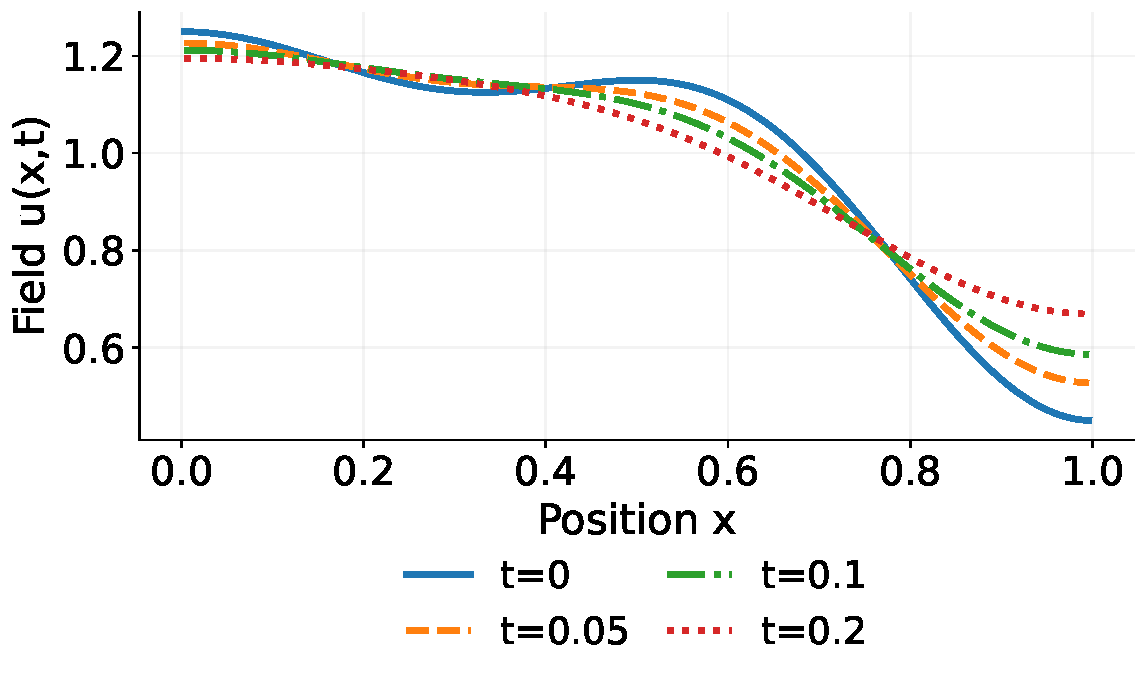
\includegraphics[width=.98\linewidth,height=.69\textheight,keepaspectratio]{presentation-figures/operator-family-panel-1.pdf}\end{frame}
\renewcommand{\notestarget}{notes.pdf\#note-functions-sampled-fields-and-input-families}
\begin{frame}[label=slide-a-function-and-its-representation-panel-2]{A parameter changes the map}
\centering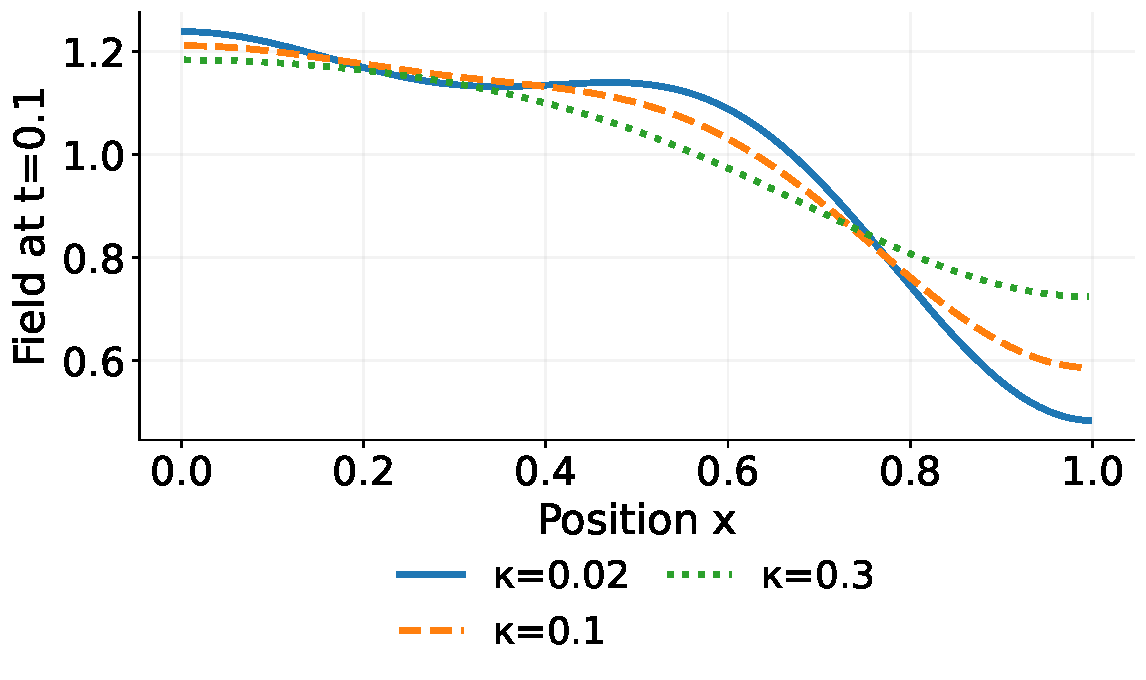
\includegraphics[width=.98\linewidth,height=.69\textheight,keepaspectratio]{presentation-figures/operator-family-panel-2.pdf}\end{frame}
\renewcommand{\notestarget}{notes.pdf\#note-functions-sampled-fields-and-input-families}
\begin{frame}[t,fragile,label=slide-a-function-and-its-representation]{A function and its representation}
\[u_0\in\mathcal F_K=\operatorname{span}\{1,\cos(\pi x/L),\ldots,\cos(K\pi x/L)\}.\]\pause{} Sampling changes the array length, not the underlying finite coefficient family.
\end{frame}
\renewcommand{\notestarget}{notes.pdf\#note-the-neumann-heat-solution-by-cosine-expansion}
\begin{frame}[t,fragile,label=slide-the-sealed-heat-equation]{The sealed heat equation}
\[u_t=\kappa u_{xx},\qquad u_x(0,t)=u_x(L,t)=0.\]\pause{} The domain, boundary conditions and diffusivity define the evolution problem.
\end{frame}
\renewcommand{\notestarget}{notes.pdf\#note-the-neumann-heat-solution-by-cosine-expansion}
\begin{frame}[t,fragile,label=slide-cosines-satisfy-the-boundary-conditions]{Cosines satisfy the boundary conditions}
\[\partial_x\cos(k\pi x/L)=-\frac{k\pi}{L}\sin(k\pi x/L).\]\pause{} The derivative vanishes at both endpoints.
\end{frame}
\renewcommand{\notestarget}{notes.pdf\#note-the-neumann-heat-solution-by-cosine-expansion}
\begin{frame}[t,fragile,label=slide-separate-one-mode]{Separate one mode}
\[u(x,t)=a_k(t)\cos(k\pi x/L)\quad\Longrightarrow\quad\dot a_k=-\kappa(k\pi/L)^2a_k.\]\pause{} Each amplitude obeys scalar exponential decay.
\end{frame}
\renewcommand{\notestarget}{notes.pdf\#note-the-neumann-heat-solution-by-cosine-expansion}
\begin{frame}[t,fragile,label=slide-the-exact-solution-operator]{The exact solution operator}
\[u(x,t)=a_0+\sum_{k=1}^K a_k e^{-\kappa(k\pi/L)^2t}\cos(k\pi x/L).\]\pause{} Higher modes decay faster.
\end{frame}
\renewcommand{\notestarget}{notes.pdf\#note-the-neumann-heat-solution-by-cosine-expansion}
\begin{frame}[t,fragile,label=slide-mean-preservation]{Mean preservation}
\[\mathcal M[u]=\frac1L\int_0^L u\,\mathrm dx=a_0.\]\pause{} The zero mode is unchanged even as all nonconstant modes decay.
\end{frame}
\renewcommand{\notestarget}{notes.pdf\#note-the-neumann-heat-solution-by-cosine-expansion}
\begin{frame}[t,fragile,label=slide-decay-of-the-nonconstant-energy]{Decay of the nonconstant energy}
\[\|u-a_0\|_{L^2}^2=\frac L2\sum_{k\ge1}a_k^2e^{-2\kappa(k\pi/L)^2t}.\]\pause{} For $\kappa\ge0$, each term is nonincreasing.
\end{frame}
\renewcommand{\notestarget}{notes.pdf\#note-generator-flow-and-observation-maps}
\begin{frame}[t,fragile,label=slide-the-generator]{The generator}
\[\mathcal A_\kappa[u]=\kappa u_{xx}.\]\pause{} It maps a current field to its instantaneous derivative, subject to the boundary domain.
\end{frame}
\renewcommand{\notestarget}{notes.pdf\#note-generator-flow-and-observation-maps}
\begin{frame}[t,fragile,label=slide-the-flow-and-its-semigroup-property]{The flow and its semigroup property}
\[\Phi_t^\kappa=e^{t\mathcal A_\kappa},\qquad\Phi_s^\kappa\Phi_t^\kappa=\Phi_{s+t}^\kappa.\]\pause{} The same equation and parameters must be used in both intervals.
\end{frame}
\renewcommand{\notestarget}{notes.pdf\#note-generator-flow-and-observation-maps}
\begin{frame}[t,fragile,label=slide-an-observable-is-another-map]{An observable is another map}
A field at one time, its complete trajectory and its mean are different outputs.\pause{} Correctly predicting the mean does not identify the nonconstant evolution.
\end{frame}
\renewcommand{\notestarget}{notes.pdf\#note-complete-case-data-partitions}
\begin{frame}[label=slide-split-complete-evolution-cases-panel-1]{Cases are complete functions}
\centering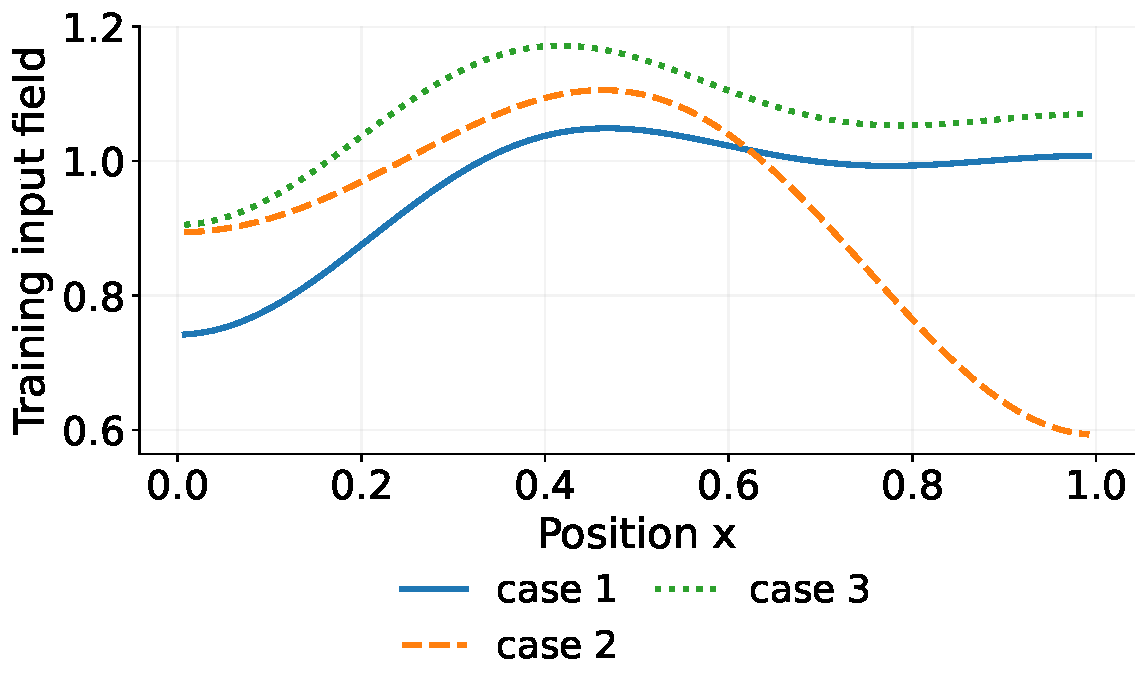
\includegraphics[width=.98\linewidth,height=.69\textheight,keepaspectratio]{presentation-figures/dataset-regimes-panel-1.pdf}\end{frame}
\renewcommand{\notestarget}{notes.pdf\#note-complete-case-data-partitions}
\begin{frame}[label=slide-split-complete-evolution-cases-panel-2]{Split by case, not mesh node}
\centering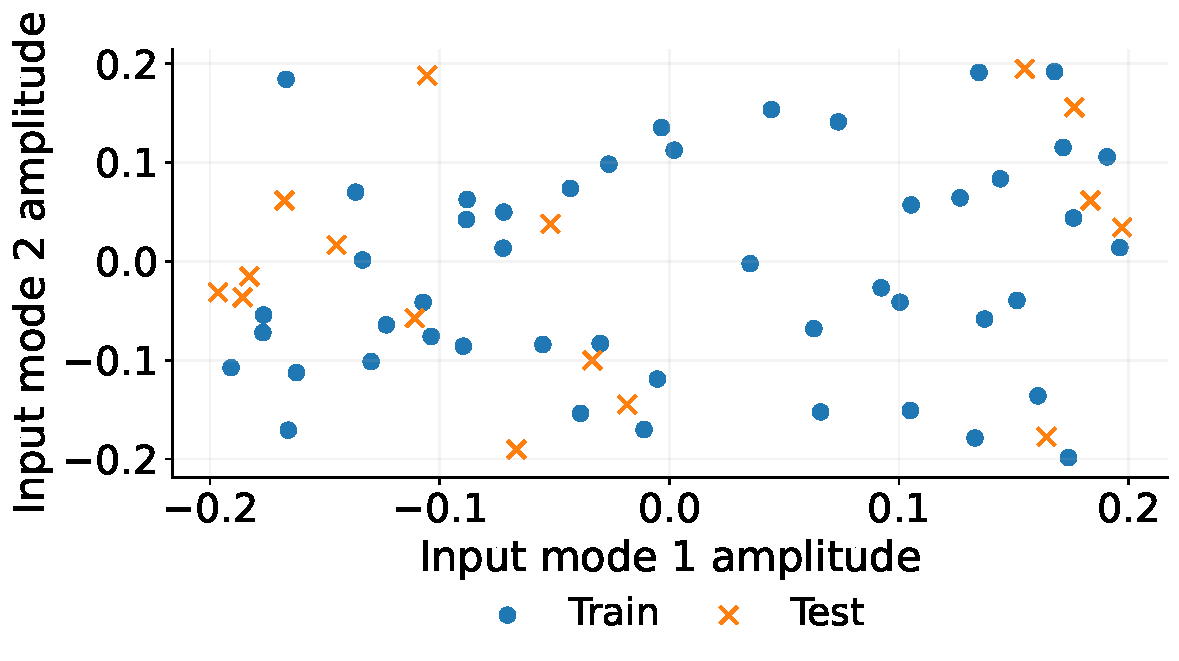
\includegraphics[width=.98\linewidth,height=.69\textheight,keepaspectratio]{presentation-figures/dataset-regimes-panel-2.pdf}\end{frame}
\renewcommand{\notestarget}{notes.pdf\#note-complete-case-data-partitions}
\begin{frame}[t,fragile,label=slide-split-complete-evolution-cases]{Split complete evolution cases}
One coefficient vector and all its snapshots remain together.\pause{} Neighboring times and spatial samples from one trajectory are not new independent cases.
\end{frame}
\renewcommand{\notestarget}{notes.pdf\#note-discrete-diffusion-and-independent-reference-solutions}
\begin{frame}[t,fragile,label=slide-the-discrete-cosine-decay-rate]{The discrete cosine decay rate}
\[\lambda_{k,h}=\frac{4\kappa}{\Delta x^2}\sin^2\left(\frac{k\pi}{2N}\right).\]\pause{} This tends to $\kappa(k\pi/L)^2$ for fixed $k$ as the grid is refined.
\end{frame}
\renewcommand{\notestarget}{notes.pdf\#note-discrete-diffusion-and-independent-reference-solutions}
\begin{frame}[t,fragile,label=slide-separate-space-and-time-error]{Separate space and time error}
\[e^{-t\lambda_{k,h}}\quad\text{versus}\quad e^{-t\kappa(k\pi/L)^2}\]\pause{} isolates space;\[ (1+\Delta t\lambda_{k,h})^{-n}\quad\text{versus}\quad e^{-t\lambda_{k,h}}\] isolates time.
\end{frame}
\renewcommand{\notestarget}{notes.pdf\#note-finite-family-prediction-and-broader-operator-claims}
\begin{frame}[t,fragile,label=slide-grid-transfer-and-parameter-transfer]{Grid transfer and parameter transfer}
A new grid can sample the same function family and operator.\pause{} A new diffusivity changes the attenuation itself; successful grid reuse does not establish parameter transfer.
\end{frame}
\renewcommand{\notestarget}{notes.pdf\#note-finite-family-prediction-and-broader-operator-claims}
\begin{frame}[t,fragile,label=slide-closed-state-and-effective-closure]{Closed state and effective closure}
The heat field is a closed autonomous state.\pause{} Omitting ionic variables from a voltage evolution can instead produce a learned effective closure limited to its trajectory distribution.
\end{frame}
\end{document}
